\chapter{Aktueller Stand der Forschung und Praxis (generell auch wiedergeben von aktuell existierenden Lösungsmustern)}

\section{Ressourcenverbrauch bei KI-Modellen}
\subsection{Ressourcenverbrauch bei KI-Modellen}
\subsubsection{Nachhaltigkeit}
\subsubsection{Stromverbrauch}
\subsubsection{Rechenleistung begrenzt, KI-Modelle wachsen schneller als verfügbare Leistung}

\section{Deep Neural Network - Boltzmann Maschinen (Erstmal DNN erklären generell)}

(Erklären von Deep Neurol Network und Neurol Network) -> Anwendungsbereiche Spracherkennung, Image recognition
Solche Deep Neural Networks, sind sehr ressourceneffizient und möglicher Forschungsbereich für Nutzung des Hardwarebeschleunigers
Idee dabei, die repräsentationspower von energybased model höher als bei LLMs, mit weniger Neuronen besser als LLMs 


Some regression tasks within computer vision in \ac{DNN} include object detection, medical image registration, head- and body-pose estimation, age estimation and visual tracking.\footcite[Vgl.][325-326]{gustafssonEnergyBasedModelsDeep2020}

->RBMs einführen und sagen warum Training vereinfacht ist

\subsection{Energy-based models}


An \ac{EBM} is a type of statistical model where the likelihood of a particular state is determined by an energy function.\footcite[Vgl.][2]{huembeliPhysicsEnergybasedModels2022}
Since 1982, those models have been continuously emerging in the machine learning field when J.J. Hopfield introduced the Hopfield Network.\footcite[Vgl.][]{hopfieldNeuralNetworksPhysical1982}
Current developments include their use in reinforcement learning, potential replacements for discriminators in generative adversarial networks and for quantum \ac{EBM}s.\footnote{Vgl.\cite{verdonQuantumHamiltonianBasedModels2019}, p. 1; Vgl.\cite{duModelBasedPlanning2021}, p. 1}
The underlying idea behind \ac{EBM}s is to establish a probabilistic physical system that is able to learn and memorize patterns but most importantly generalize it.\footcite[Vgl.][2]{huembeliPhysicsEnergybasedModels2022} 
Especially, it involes learning an energy function \(E_{\theta}(x) \in \mathbb{R}\) and assigning the low energy to observed data \(x_i\) and high energy to other values \(x\).\footcite[Vgl.][330]{gustafssonEnergyBasedModelsDeep2020}
\begin{figure}[H]
    \centering
    \fbox{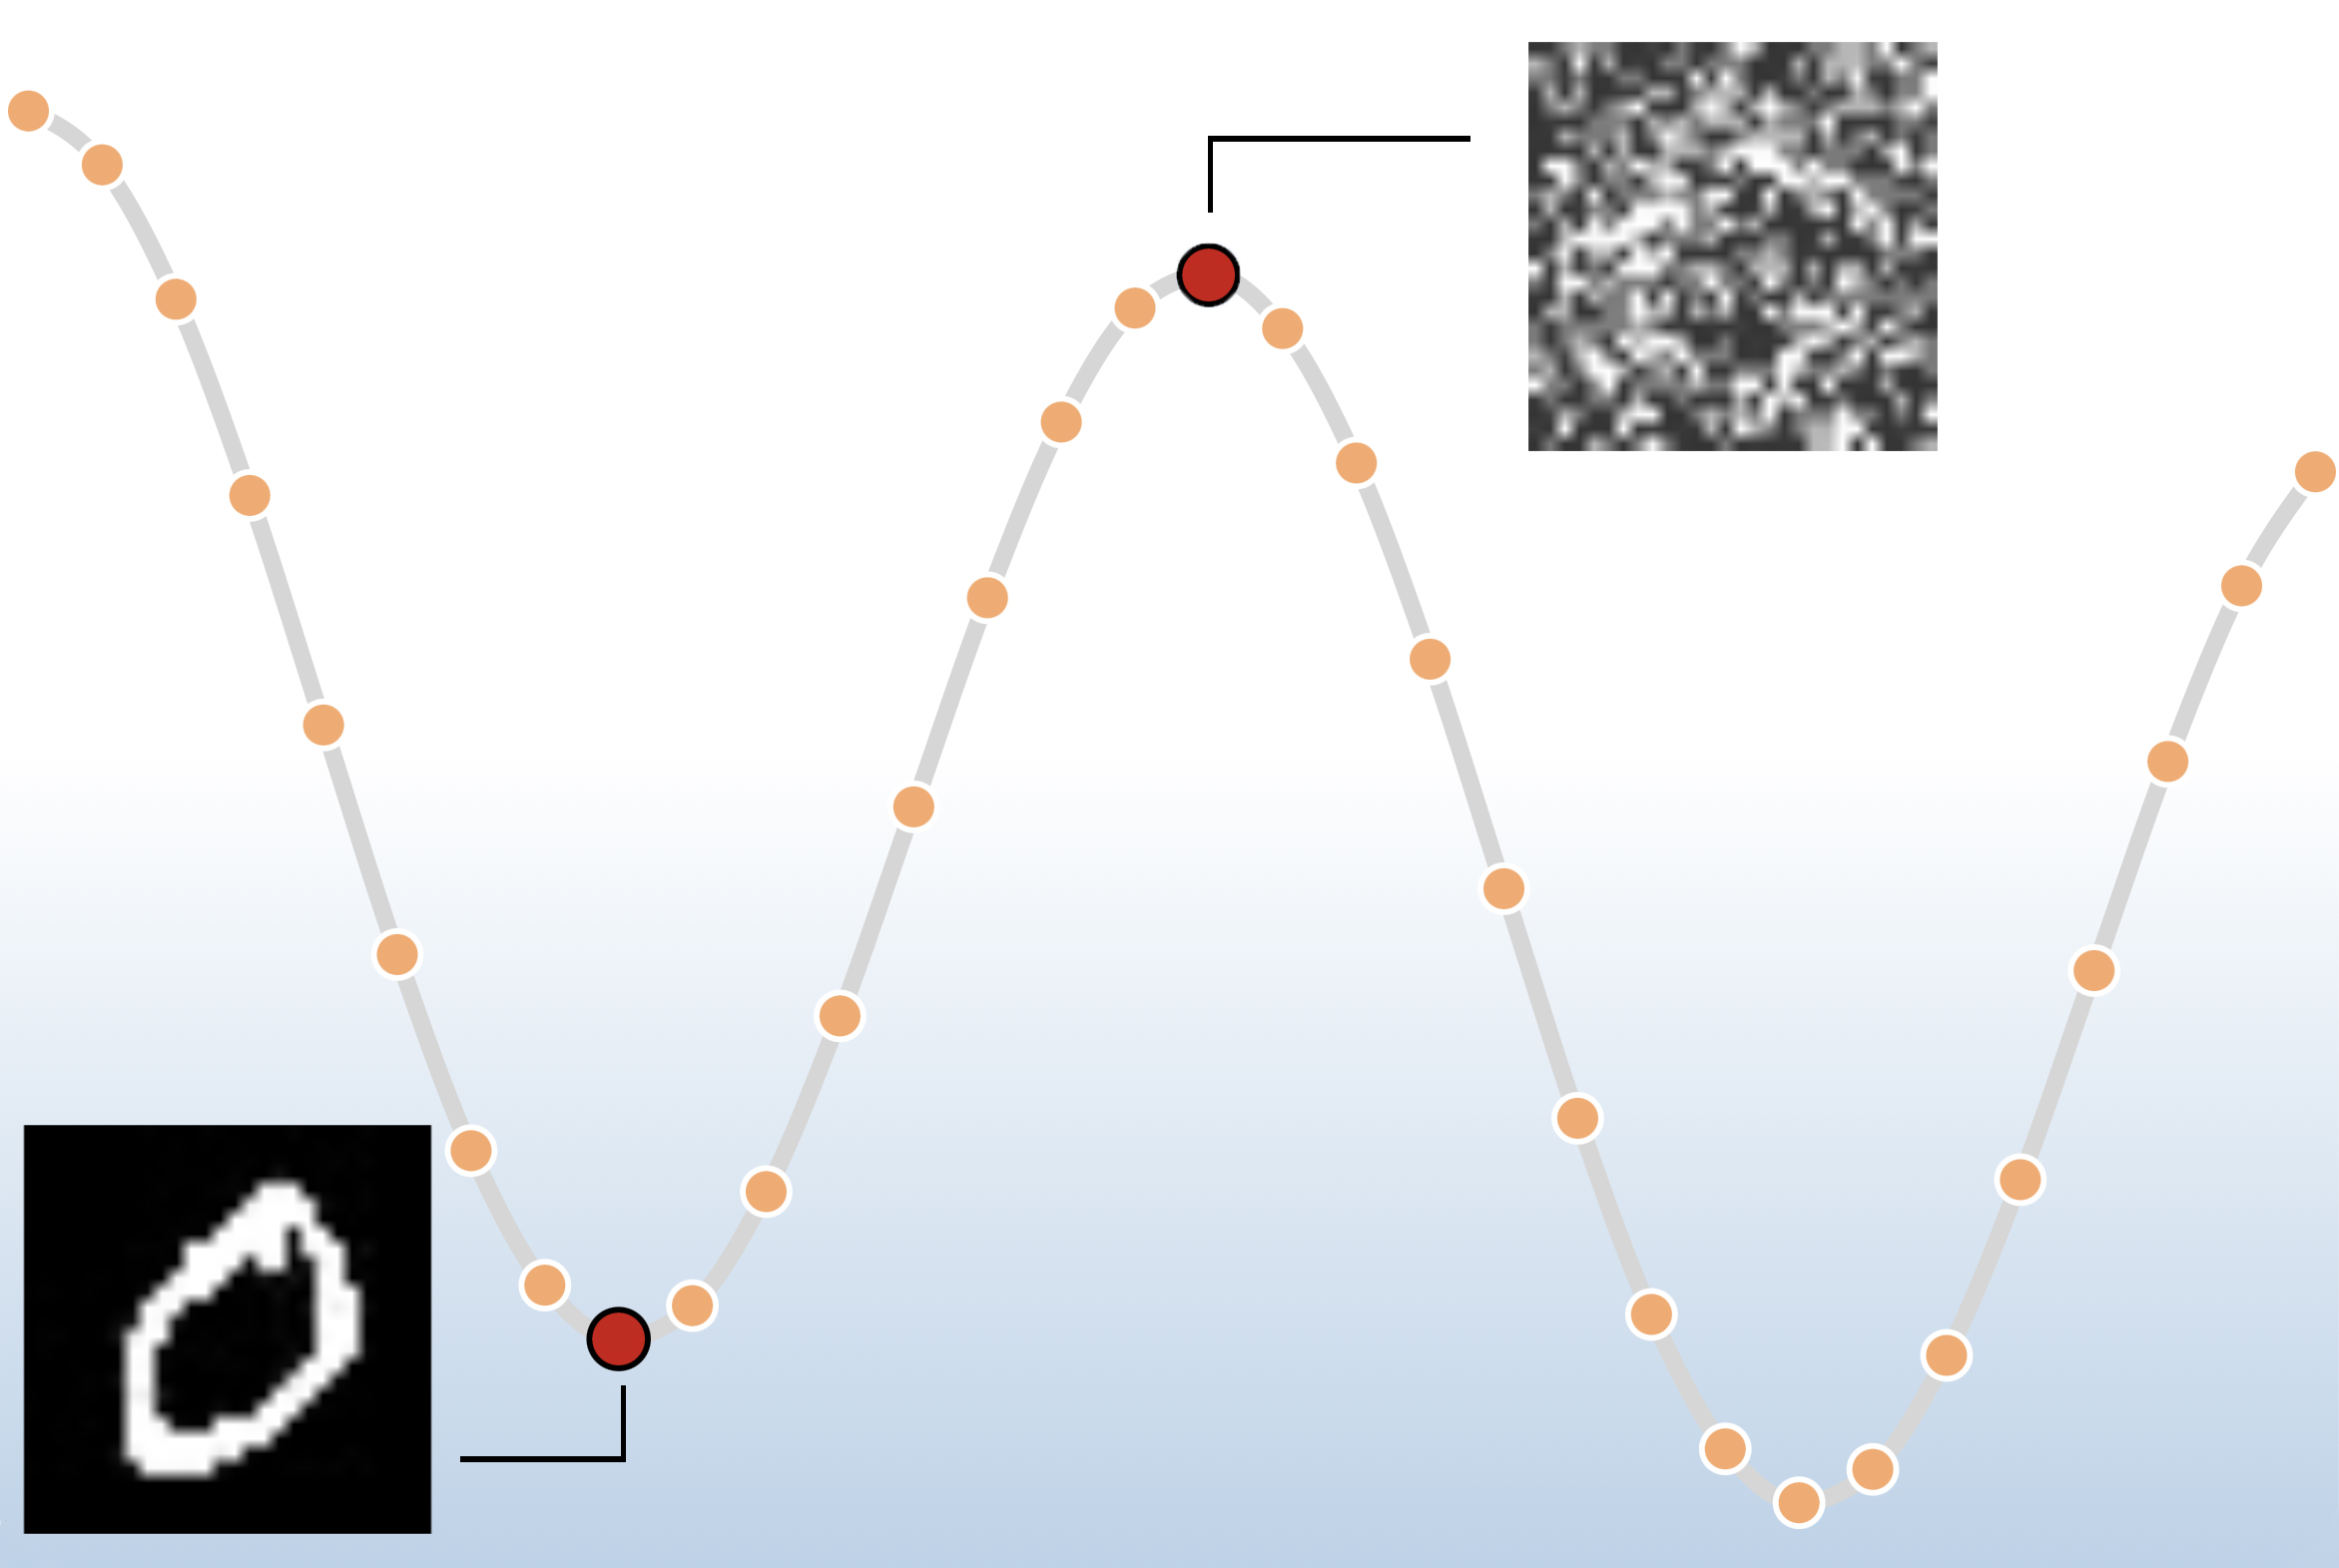
\includegraphics[width=0.4\linewidth]{graphics/energielandschaft.jpg}}
    \caption{Figure of a logistic sigmoid function \ac{RBM}}
\end{figure}
In this figure a simplified energy landscape is shown where the local minima correspond to states that encode an MNIST digit.\footcite[Vgl.][6]{huembeliPhysicsEnergybasedModels2022} It is visible that observed data settles in the local minimum of the energy landscape, in this case a clear 0. On the other hand close to the local maxima of the energy landscape the 0 is only barely recognizable and therefore got a higher energy value assigned to it.
The assumption of the underlying distribution function \( P(x) \)  is equal to the solution of the optimization problem:
\begin{equation}
    P(x) = \frac{1}{Z} \exp\left(-\frac{E(x)}{T}\right),
\end{equation}
where \( Z \) is given by the partition function to ensure
that the density function normalizes to a total probability of 1 and \( T \) is interpreted as the temperature .\footcite[Vgl.][2-3]{huembeliPhysicsEnergybasedModels2022}
As a result the behavior of a \ac{EBM} is determined by 2.2. 
The aim of the training is to match the real data \( P_{\text{data}} \) as closely as possible with the internal model \( P_{\text{model}} \).
A practical method to achieve this goal is to use the KL divergence. KL divergence is a mathematical equation that helps to meassure how close the predictions are by comparing the model's learned distribution to the true distribution of the data:
\begin{equation}
    G = \sum_x P^+(x) \ln \left( \frac{P^+(x)}{P^-(x)} \right)
\end{equation}
Here, \(P^+(x)\) is the probability when the states are determined by a data input from the environmnet, while \(P^-(x)\) represents the internal network running freely, also referred to as ``dreaming''.\footcite[Vgl.][154-155]{ackleyLearningAlgorithmBoltzmann1985}
To optimise the KL divergence, in this case \( G \), the energy is adjusted, whereby data is assigned to low energy states (according to 2.1) and the training data receives high energy and therefore high probabiliies.\footcite[Vgl.][2-3]{zhaiDeepStructuredEnergy2016}
To complete the section the ``partition function'', \( Z \), used in 2.1 is given by summing over all possible pairs of visible and hidden vectors:
\begin{equation}
    Z = \sum_x \exp\left(-\frac{E(x)}{T}\right)
\end{equation}
As a side note that is worth mentioning is, that using the maximum likelihood estimator for \( Z \) is impractical due to the requirement of summing over all possible states, which leads to an exponential increase in the number of states for larger systems.\footcite[Vgl.][2-3]{zhaiDeepStructuredEnergy2016}

\subsection{concept Boltzmann Maschine and usage of the model}

A \ac{BM} is a specific symmetrical \ac{EBM} consisting of binary neurons \{0, 1\}.\footcite[Vgl.][260]{amariInformationGeometryBoltzmann1992}
The neurons of the network can be split into two functional groups, a set of visible neurons and a set of hidden neurons.\footcite[Vgl.][154]{ackleyLearningAlgorithmBoltzmann1985}
Therefore, the \ac{BM} is a two-layer model with a visible layer (``v'') and a hidden layer (``h'').\footcite[Vgl.][448]{salakhutdinovDeepBoltzmannMachines2009}
The visible layer is the interface between the network and the environment. It receives data inputs during training and sets the state of a neuron to either \{0, 1\} which represents activated or not activated.
On the other hand, the hidden units are not connected to the environment and can be used to “explain” underlying constraints in the internal model of input vectors and they cannot be represented by pairwise constraints.\footcite[Vgl.][154]{ackleyLearningAlgorithmBoltzmann1985}
The connection between the individual neurons is referred to as bidirectional, as each neuron communicates with each other in both directions.\footcite[Vgl.][149]{ackleyLearningAlgorithmBoltzmann1985}

As early as 1985, one of the founding fathers of artificial intelligence, ``Geoffrey Hinton'', was aware that an \ac{BM} is able to learn its underlying features by looking at data from a domain and developing a generative internal model.\footcite[Vgl.][148]{ackleyLearningAlgorithmBoltzmann1985}
In the next step, it is possible to generate examples with the same probability distribution as the input data examples shown.
In the following figure \ref{fig1}, a general \ac{BM} is depicted, where the upper layer embodies a vector of stochastic binary 'hidden' features, while the lower layer embodies a vector of stochastic binary 'visible' variables.\footcite[Vgl.][449]{salakhutdinovDeepBoltzmannMachines2009}

\begin{figure}[H]
    \centering
    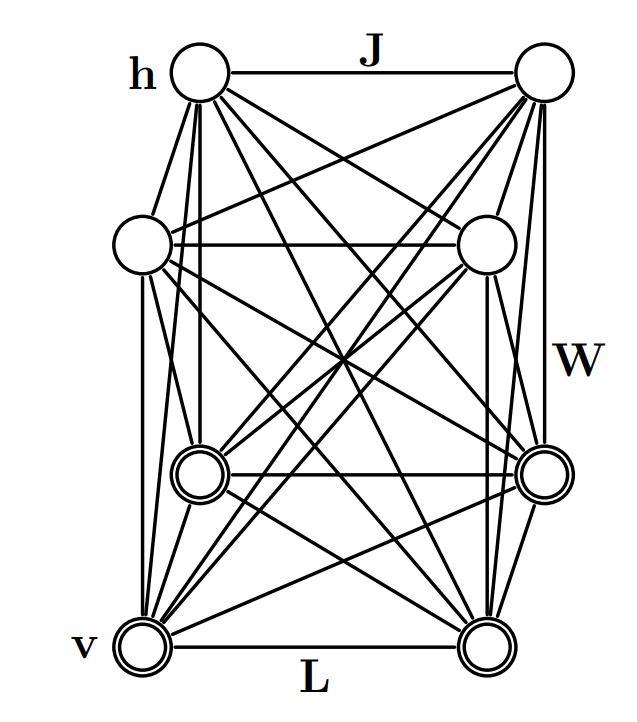
\includegraphics[width=0.25\linewidth]{graphics/General_BM.png}
    \caption{figure of a general Boltzmann Machine}
    \label{fig1}
\end{figure}
The model contains a set of visible units \( v \in \{0, 1\} \), and a set of hidden units \( h \in \{0, 1\} \) (see Fig. 1). The energy function of the \ac{BM} with the states \( \{v, h\} \) is defined as:
\begin{equation}
E(v, h; \theta) = -\frac{1}{2} v^T L v - \frac{1}{2} h^T J h - v^T W h,
\end{equation}

where \( \theta = \{W, L, J\} \) are the model parameters.\footcite[Vgl.][448]{salakhutdinovDeepBoltzmannMachines2009}
\( W, L, J \) represent visible-to-hidden, visible-to-visible and hidden-to-hidden weights.
The individual neurons can be made to try to minimize the global energy by setting the right assumptions.\footcite[Vgl.][150]{ackleyLearningAlgorithmBoltzmann1985}
Entering a particular input to the machine, the system will find the minimum energy configuration that can illustrate the input.\footcite[Vgl.][150]{ackleyLearningAlgorithmBoltzmann1985}
A simple method to find a local energy minimum is to switch into wichever of the two states of a neuron hold the lower energy given the current state of the other neurons.\footcite[Vgl.][110]{fahlmanMassivelyParallelArchitectures1983}  
The exact reason for this is the following: ``If all the connection strengths are
symmetrical, which is typically the case for constraint satisfaction
problems, each unit can compute its effect on the total energy from
information that is locally available.''\footcite[110]{fahlmanMassivelyParallelArchitectures1983}  
By inserting the function 2.4 into the earlier introduced KL-divergence 2.2 and doing gradient descend the following learning rule to update the weights and biases results\footcite[Vgl.][5]{hintonPracticalGuideTraining2012}:

\begin{equation}
    \Delta w_{ij} = \epsilon ( \langle v_i h_j \rangle_{\text{data}} - \langle v_i h_j \rangle_{\text{model}} )
\end{equation}

The network can now update the weights ``W'' that exist between the neurons through the training rule based on the observations that served as input and modified by the learning rate \(\epsilon\).\footcite[Vgl.][1-2]{barraEquivalenceHopfieldNetworks2012}

Performing exact maximum likelihood learning in this model is intractable because exact computation of the data predictions and the model predictions takes a time that is exponential in the number of hidden units.\footcite[Vgl.][449]{salakhutdinovDeepBoltzmannMachines2009}
When the number of hidden units is large compared to the number of visible units it is impossible to achieve a perfect model because of the totally connected network and the resulting \( 2^n \) possbilities.\footcite[Vgl.][154]{ackleyLearningAlgorithmBoltzmann1985}
This leads back to the briefly mentioned constraint of equation 2.3, that is needed to calculate an activation probability of a neuron, which is required to update a weight in the training process shown in 2.5.

A specific example to demonstrate why it is intractable to calculate a activiation of a \ac{BM} is the following. The \ac{BM} has 80 visible nodes and 120 hidden nodes and therefore the possbilities of states of neurons are \( 2^{200} \), which is \( 1.61 \times 10^{60}\). 
To put this in perspective the toal atoms that exist on earth are only estimated to be around \( 1.33 \times 10^{50}\).\footnote{Vgl.\cite{helmenstineHowManyAtoms2022}, p. 478-480; Vgl.\cite{schlammingerCoolWayMeasure2014}, p. 1}
That means even if it would be possible to store one information per atom it would just not be enough. 

\subsection{Training of Restriced Boltzmann Machines}

As a solution for the training problem Hinton and Sejnowski proposed Gibbs sampling as an algorithm to aporoximate both expectations.\footcite[Vgl.][158-165]{ackleyLearningAlgorithmBoltzmann1985}
Furthermore, the intralayer connections of the model got removed and the result is the so called \ac{RBM}.
To transform an \ac{BM} into a \ac{RBM} the diagonal elements \( L \) and \( J \)  introduced earlier, are set to 0 and as a result the well-known model of a \ac{RBM} establishes shown in fig.2.\footcite[Vgl.][449]{salakhutdinovDeepBoltzmannMachines2009}

\begin{figure}[H]
    \centering
    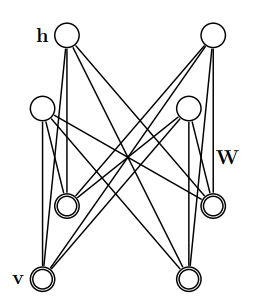
\includegraphics[width=0.25\linewidth]{graphics/RBM_Modell.png}
    \caption{Figure of a \ac{RBM}}
\end{figure}
What can be recognized that no more visible-to-visible and hidden-to-hidden connections can be found in the model.
The configuration of the visible and hidden units \( (v, h) \) therefore has also an updated energy function (Hopfield, 1982) given by:
\begin{equation}
E(v, h) = - \sum_{i \in \text{visible}} a_i v_i - \sum_{j \in \text{hidden}} b_j h_j - \sum_{i,j} v_i h_j w_{ij},
\end{equation}
where \( v_i, h_j \) are the binary states of a visible unit \( i \) and hidden unit \( j \), \( a_i, b_j \) are their biases and \( w_{ij} \) is the weight between them.\footcite[Vgl.][3-4]{hintonPracticalGuideTraining2012a}
Despite, compared to the fully connected \ac{BM} the \ac{RBM} is less complex the advantages of training surpasses the loss in expressivity.\footcite[Vgl.][4]{huembeliPhysicsEnergybasedModels2022}
The \ac{RBM} has recently been drawing attention in the machine learning community beceause of its adaption and extention for various tasks such as representational learning, document modeling, image recognition and for
serving as foundational components for deep networks including Deep Boltzmann Machine, Deep Belief Networks and hybrid models with CNNs.\footcite[Vgl.][1186]{zhangOverviewRestrictedBoltzmann2018}
The training of the model can be split up into the following steps:

\textbf{1. Forward Pass (positive phase)}

During the forward pass, the visible units are set to an input of the training data. Next up the hidden units are computed.
The computation of the hidden units involves calculating their acitivation probabilities and performing an actual sampling with their calculated activation probabilities.
With the \ac{RBM} it is now easy to get an analytical calculated unbiased sample of $(\textbf{v}_i\textbf{h}_j)_{data}$.\footcite[Vgl.][5]{hintonPracticalGuideTraining2012}
Given a input data out of the training images, \( v \), the binary state, \( j \), of each hidden unit,  \( h_j \), is set to 1 with following probability:

\begin{equation}
p(h_j = 1 | \textbf{v}) = \sigma(b_j + \sum_i v_i w_{ij}),
\end{equation}
where $\sigma(x)$ is the logistic sigmoid function is then an unbiased sample. The sigmoid function is defined as $\sigma(x) = \frac{1}{1 + \exp(-x)}$ and shown in figure 4:
\begin{figure}[H]
    \centering
    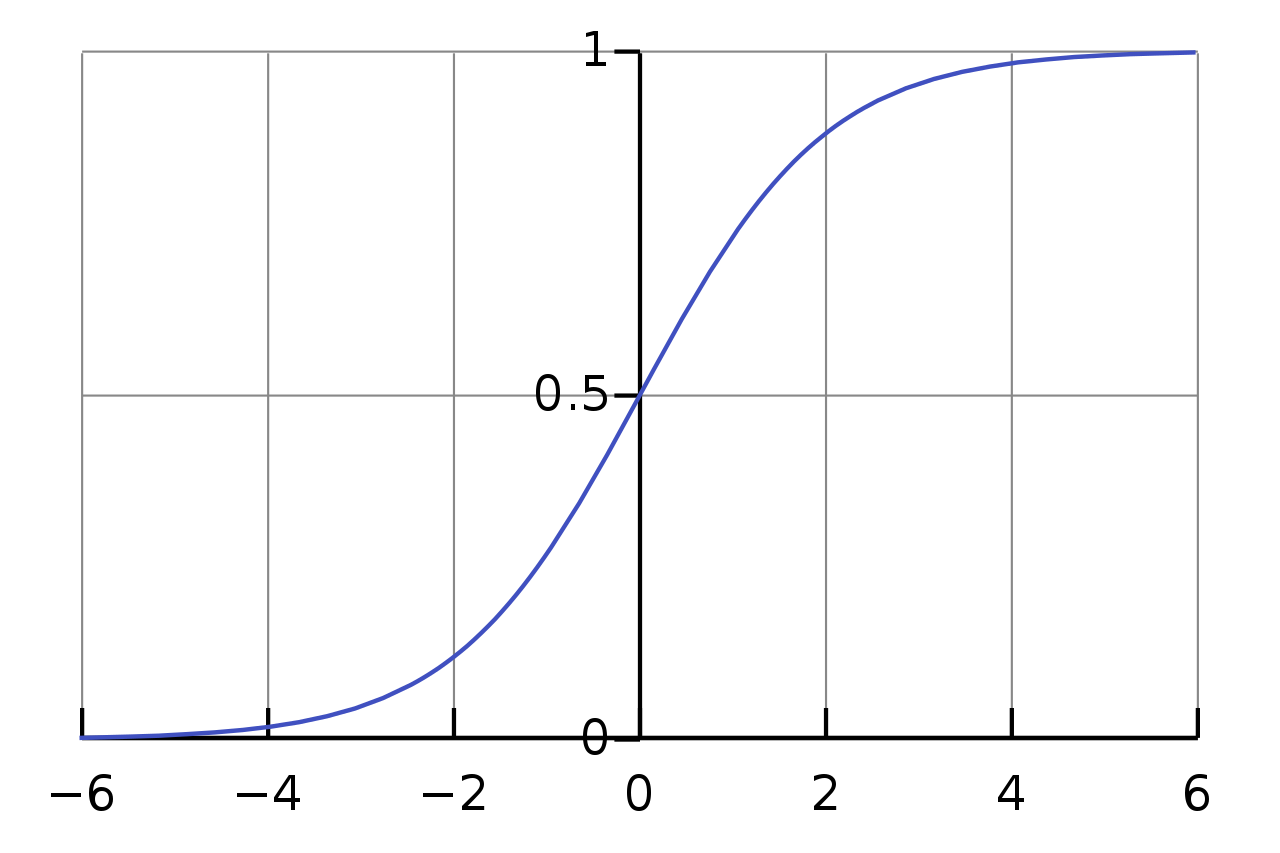
\includegraphics[width=0.5\linewidth]{graphics/logistic_sigmoid.png}
    \caption{Figure of a logistic sigmoid function \ac{RBM}}
\end{figure}
The result is a set of probabilities that reflects how likely it is for each hidden unit to be on or off given the input data.\footcite[Vgl.][6]{huembeliPhysicsEnergybasedModels2022}
The sampling part of the positive phase uses the just calculated acitivation probabiliy of each hidden unit and performs a random experiment with it.
Afterwards, the hidden unit is either activated or not activated and the training process continues with the new state of the hidden units (activated or not activated).

\textbf{2. Reconstruction (negative phase)}

In this phase, the sampled hidden states are used to reconstruct the visible units. 
This is essentially a prediction of the input, which is calulated with following probability:\footcite[Vgl.][6]{hintonPracticalGuideTraining2012}
\begin{equation}
    p(v_i = 1 | \mathbf{h}) = \sigma(a_i + \sum_j h_j w_{ij})
\end{equation}
The sampling part of the negative phase uses the just calculated acitivation probabiliy
of each visible unit and performs a random experiment, like in the positive phase.
Now, the result is a prediction of the input in the visible nodes.
Afterwards, a half forward pass is made to calculate the activation probability of a hidden unit again based on the activated or not activated visible units.

\textbf{3. Weight update}

Meanwhile, all the requirements to update the weights are satisfied and can be used within the equation 2.5. 
The delta that results is summed to the current weight and therefore the internal model gets closer to prediciting the observed data.
Therefore, one training Iteration consisting of 1 Forward Pass, 1 Reconstruction and 0.5 Forward Pass again is accomplished.
Repeating this training steps \( N \) times for a suitable chosen \( N \) the model learns better, since more steps of alternating Gibbs sampling were performed.\footcite[Vgl.][6]{huembeliPhysicsEnergybasedModels2022}




\subsubsection{Markov-Chain-Monte-Carlo-Verfahren}
Metropolis Hastings,
Conrtrastive Divergence

\subsection{Aktuelle Probleme mit RBM/BM}


Exact maximum likelihood learning in the Boltzmann machine is infeasible due to the exponentially increasing computation time with the number of hidden units.
Hinton and Sejnowski's 1983 algorithm approximates this via Gibbs sampling, but it is limited by the significant time needed to reach the stationary distribution in a complex, multimodal energy landscape.

\section{Hardwarebeschleuniger}
\subsection{Aktuelle Ansätze im Bereich KI und weitere Lösungen}
\subsubsection{Asics}
\subsubsection{Quantencomputing}
\subsection{ISING Maschine/ Physikinspirierter Hardwarebeschleuniger}
\subsubsection{Konzept (mit Energiefunktion), Probleme der Digitalrechner bzw. Unterschied zu Digitalrechner}
\subsubsection{Aktuelle Anwendung}
\subsubsection{Potentielle Einsatzgebiete für KI-Modelle}
\subsubsection{Parallelen Energiefunktion BM und ISING Maschine}

\section{Memristor Hopfield Network}
\subsection{Memristor}
\subsection{Hopfield Network}
\subsection{Crossbar}
\subsection{Output Hopfield Networtk}
\subsection{Noisy HNN}
